\documentclass[a4paper,spanish]{article}
\usepackage[spanish]{babel}
\usepackage[utf8]{inputenc}	%para los acentos
\usepackage{caratula}
\usepackage{amsmath, amscd, amssymb, amsthm, latexsym, verbatim}
\usepackage{graphicx, graphics, caption}
\usepackage{fancyhdr}
% \usepackage{float, algorithmic}
% \usepackage[a4paper=true]{hyperref}
% \usepackage{algorithm}
\usepackage{multirow}

%probando para los margenes
\usepackage[top= 3cm, bottom= 3cm , left= 2.5cm, right= 2.5 cm]{geometry}

% configuro el paquete de algoritmos
% \floatname{algorithm}{Algoritmo}

\makeatletter
\newcounter{algorithmic}
\let\ORIG@algorithmic\algorithmic
\def\algorithmic{\stepcounter{algorithmic}\ORIG@algorithmic}
\def\theHALC@line{\thealgorithmic-\theALC@line}
\def\theHALC@rem{\thealgorithmic-\theALC@rem}
\makeatother

% encabezados
\newcommand{\norma}[1]{\left|\left|#1\right|\right|}
\parskip=1ex
\pagestyle{fancy}
\pagenumbering{arabic}
%\fancyhf{}
\renewcommand{\headrulewidth}{0.02 cm}
\renewcommand{\footrulewidth}{0 cm}
\rhead{Animal}
\lhead{Seguridad de la Información}
\def\septad{\rule{16 cm}{.2 mm}}
\usepackage{hyperref}

% defino un environment propio para las ecuaciones
%\newenvironment{ecuacion}
%	{\begin{equation} \begin{aligned}}
%	{\end{aligned} \end{equation}}
%	
%\newenvironment{ecuacion*}
%	{\begin{equation*} \begin{aligned}}
%	{\end{aligned} \end{equation*}}

% comienzo el documento
\begin{document}
	\materia{Seguridad de la Información}

\titulo{Animal}

\integrante{Mauricio Alfonso}{65/09}{mauricioalfonso88@gmail.com}
\integrante{Andres Ispani}{530/04}{andyispani@gmail.com}
\integrante{Ezequiel Gutesman}{715/02}{egutesman@gmail.com}
\integrante{Daniel Foguelman}{}{dj.foguelman@gmail.com}


\maketitle


	\tableofcontents
	\section{Animal}
	\subsection{Android ADT Bundle} 
	
	\subsection{Genymotion Android Emulator}

	\subsection{Sinatra}
	\section{Animal}

	\subsection{Descripción}

	Animal es un malware de android que se encarga de robar las fotos del teléfono y subirlas a un servidor nuestro. 

	\subsection{Permisos requeridos}
		\begin{itemize}
			\item \texttt{android.permission.INTERNET} para acceder a internet y subir las fotos.
			\item \texttt{android.permission.ACCESS\_NETWORK\_STATE} para saber si hay wi-fi disponible.
		\end{itemize}

	\subsection{Implementación}

		\subsubsection{MainActivity}
			Animal crea una actividad de android \footnote{ \url{http://developer.android.com/reference/android/app/Activity.html} } en \texttt{MainActivity}, que busca en la tarjeta SD archivos que sean fotos sacadas con la cámara del teléfono. Para eso busca en 3 directorios donde suelen haber fotos (\texttt{DCIM/Camera}, \texttt{Pictures} y \texttt{Downloads}) archivos con nombres de fotos (que empiecen con \texttt{IMG} o \texttt{DSC} y tengan \texttt{jpg}, \texttt{png} o \texttt{jpeg} como extensión). Una vez que encontró todos las fotos ejecuta varios threads de la tarea asincrónica \texttt{FileUploader}, que se encarga de subir una foto cada uno. Los threads se acumulan en una cola de manera que no haya más de uno corriendo al mismo tiempo. Una vez que terminó de agregar una llamada a ejecución de \texttt{FileUploader} por cada foto, cierra la actividad haciendo una llamada al método \texttt{finish()}. De esta manera cuando el usuario abre la aplicación, ésta se cierra casi inmediatamente pero \texttt{FileUploader} sube las fotos en segundo plano. 

		\subsubsection{FileUploader}
			Cada thread de la tarea asincrónica \texttt{FileUploader} se encarga de subir la foto que reciba, haciendo un \texttt{POST} \texttt{HTTP} hacia nuestro servidor. Cada ejecución de un thread recibe un archivo como parámetro. Para evitar subir archivos usando 3G, \texttt{Animal} chequea si el celular está conectado a internet por wi-fi, y en caso contrario espera hasta que lo esté, chequeando el estado de conexión periódicamente. Una vez que el celular se encuentra conectado a una red wi-fi, el thread envía un \texttt{POST HTTP} a la dirección de nuestro servidor. Dicho \texttt{POST} contiene el nombre y contenido de la foto codificados en Base64 como parámetros de url \texttt{nombre} y \texttt{valor} respectivamente. El modo de codificación de Base64 no es el tradicional, sino uno conocido como \texttt{url-safe Base64} que no contiene ningún caracter no permitido en un url ni fines de línea.\\

			Como \texttt{FileUploader} es una \texttt{AsyncTask} \footnote{\url{http://developer.android.com/reference/android/os/AsyncTask.html}}, cada uno de los llamados a ejecución que se hacen se guardan en una cola y se ejecutan de manera serial, por lo tanto los POSTs no se envían todos juntos en paralelo, lo cuál sería malo para nuestro servidor y sobrecargaría la CPU del celular con threads si hubiera muchas fotos.
		
		\subsubsection{Servercito}
			El servidor escucha los POSTs que recibe a la ruta \texttt{/uploads}, decodifica el nombre y contenido del archivo y lo guarda en la carpeta \texttt{/fotos}.

	\subsection{Problemas}
		Intentamos en principio subir las fotos en Base64 a Pastebin \footnote{ \url{http://pastebin.com} } y poner una ``clave'' como nombre de las subidas, para poder encontrarlas con facilidad de manera anónima sin tener que exponer la dirección de nuestro servidor, pero nos encontramos con 2 limitaciones importantes de Pastebin: 
		\begin{itemize}
			\item Un l\'imite de tamaño de 0.5 MB nos limita a fotos muy chicas o a achicar las fotos existentes
			\item Un l\'imite de 10 subidas por d\'ia.
		\end{itemize}

		Por estas razones preferimos usar un servidor propio.


	\section{Keylogger}

	\subsection{Descripción}

	Se busca crear una aplicación maliciosa para Android que envíe a un atacante todo lo tipeado por el usuario, incluyendo nombres de usuario y passwords. Instalando un teclado personalizado, se puede facilmente loguear todo lo que se necesita. Sin embargo, los usuarios son cada vez más cuidadosos con lo que instalan, en parte gracias a avisos del sistema operativo informando de los peligros (ver Figura \ref{fig:keyboard}). Para que sus aplicaciones sean instaladas, los desarrolladores de teclados u otras aplicaciones de accesibilidad muchas veces no incluyen permisos de internet de tal forma de dar confianza (ver Figura \ref{fig:light_flow}).
	De esta forma, el objetivo es crear un teclado sin permisos de internet, que pueda enviar la información utilizando una segunda aplicación cómplice.
	
	\begin{figure}[h]
		\centering
		\begin{minipage}{.5\textwidth}
			\centering
			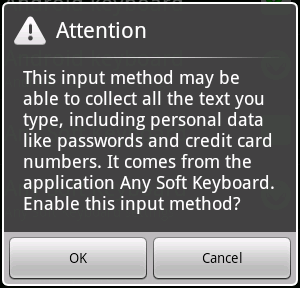
\includegraphics[width=.7\linewidth]{keyboard}
			\captionof{figure}{Warning al instalar un teclado}
			\label{fig:keyboard}
		\end{minipage}%
		\begin{minipage}{.5\textwidth}
			\centering
			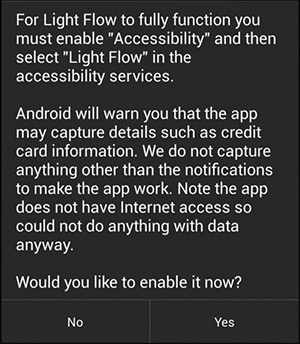
\includegraphics[width=.7\linewidth]{light_flow}
			\captionof{figure}{Ejemplo: Aplicación Light Flow avisa que sin permisos de internet no puede hacer nada con la información capturada}
			\label{fig:light_flow}
		\end{minipage}
	\end{figure}
	
	\subsection{AnimalKeyboard}
		
		\subsubsection{Permisos requeridos}
			\begin{itemize}
				\item \texttt{android.permission.BIND\_INPUT\_METHOD} Para poder registrarse como teclado. Requerido por cualquier teclado.
			\end{itemize}

		\subsubsection{Descripción}
			\emph{Animal Keyboard} es un teclado de Android que ofrece un tab de emoticones para incentivar a los usuarios a instalarlo. No tiene ning\'un permiso extra, por lo que por s\'i solo es inofensivo.	
				Al iniciarse intenta conectarse con una segunda aplicación (FunWithAnimals). Si no está instalada, no loguea nada y se comporta como cualquier teclado normal.
	
	\subsection{FunWithAnimals}
		\subsubsection{Permisos requeridos}
			\begin{itemize}
				\item \texttt{android.permission.INTERNET} Para poder bajar las fotos de animales (y enviar la información de keylogger)
			\end{itemize}
			
		\subsubsection{Descripción}
			\emph{FunWithAnimals} es una aplicación que cada vez que se abre, le ofrece al usuario una foto distinta de un gato, bajada de internet gracias a sus permisos. Si se instala por sí sola sin \emph{AnimalKeyboard}, es todo lo que hace.
			
	\subsection{AnimalKeyboard + FunWithAnimals}
	
		\subsubsection{Descripción}
		Al estar ambas aplicaciones instaladas, el procedimiento es el siguiente:
			\begin{itemize}
				\item \texttt{FunWithAnimals} registra un servicio que escucha mensajes
				\item Cada vez que se escribe una letra, \texttt{AnimalKeyboard} se la envía a \texttt{FunWithAnimals} mediante el uso de Binders \footnote{\url{http://developer.android.com/reference/android/os/Binder.html}}
				\item \texttt{FunWithAnimals} guarda las letras en un archivo
				\item Cuando el usuario abre \texttt{FunWithAnimals}, este además de bajar una foto de un gato, envía todas las letras guardadas a un servidor del atacante.
			\end{itemize}

		\subsubsection{Instrucciones}
			\begin{itemize}
				\item Instalar AnimalKeyboard.apk y FunWithAnimals.apk
				\item Ir a la configuración del teléfono
				\item Ir a Language \& input
				\item Tildar "Animal Keyboard"
				\item Ir a algún campo de texto, por ejemplo en la aplicación de SMS
				\item Arrastrar desde arriba para acceder a la barra de notificaciones
				\item Seleccionar 'Choose input method'
				\item De estar presente, apagar "Hardware physical keyboard"
				\item Activar "Animal Keyboard"
				\item El teclado nuevo debería aparecer en pantalla. Comprobar que es el correcto notando que al clickear en "123" aparece un botón nuevo de emoticones.
				\item Tipear algo
				\item Salir de la aplicación de SMS, ir al menú de aplicaciones y abrir "Fun With Animals"
				\item Se muestra en pantalla lo escrito, y se envía en segundo plano a nuestro servidor
			\end{itemize}

	\section{Instrucciones de Uso}

	\subsection{Android ADT Bundle}
		Para poder compilar las aplicaciones o agregarlas al emulador es necesario contar con el paquete Android ADT Bundle que se consigue en \url{https://developer.android.com/sdk/index.html}. El ejecutable de la interfaz Eclipse se encuentra en la carpeta eclipse. \\

		Para agregar las aplicaciones al Eclipse es necesario seleccionar la opción \texttt{File -> Import}, elegir \texttt{Android -> Existing Android code into workspace} y seleccionar el directorio de la aplicación.

	\subsection{Genymotion}
		Si bien las aplicaciones corren en el emulador incluido en el ADT Bundle, se recomienda Genymotion por razones de performance. Además como el emulador oficial no usa wi-fi, no es posible testear si funciona la app Animal (aunque si las otras), ya que Animal está diseñada para solo subir fotos sólo por wi-fi.\\

		Para usar Genymotion es necesario crear una cuenta en \url{http://www.genymotion.com/} y bajarse el instalador para el sistema operativo correspondiente. También es necesario bajarse e instalar el plugin para Eclipse. Al abrir Genymotion por primera vez es necesario bajarse un dispositivo virtual de entre los disponibles, para lo cuál será necesario loguearse con la cuenta creada.

	\subsection{Servercito}
		Para tener todo lo necesario para correr el servidor en linux es necesario

		\begin{itemize}
			\item Instalar RVM (Ruby Version Manager) 	\begin{verbatim}curl -sSL https://get.rvm.io | bash -s stable --ruby\end{verbatim}.\
			Puede que sea necesario agregar \begin{verbatim}[[ -s "$HOME/.rvm/scripts/rvm" ]] && source "$HOME/.rvm/scripts/rvm"\end{verbatim}\
	a .bashrc
			\item Instalar la versión 1.9.2 de Ruby con \begin{verbatim}rvm install 1.9.2\end{verbatim}.
			\item Instalar Sinatra con \begin{verbatim}gem install sinatra\end{verbatim}.
			\item Instalar la librería haml con \begin{verbatim}gem install haml\end{verbatim}.
		\end{itemize}

		Una vez instalado todo lo necesario debería poder correr el servidor con \texttt{ruby server.rb} en el directorio Servercito.
	
	\subsection{Direcciones IP}
		Por defecto Severcito bindea a la dirección IP \texttt{192.168.33.1} con el puerto \texttt{4567}, a la que también referencian las aplicaciones. Si esa dirección IP no está disponible, será necesario cambiarla por otra en el código de \texttt{server.rb} y también en las aplicaciones. Para cambiar la dirección del servidor en las aplicaciones es necesario modificar el archivo \texttt{server.properties} en la carpeta \texttt{assets} de cada aplicación que usa internet (todas excepto Animal Keyboard). Es necesario hacer este cambio desde Eclipse, para que al guardar el archivo recompile la aplicación con la nueva dirección. Es importante que la dirección del servidor en \texttt{server.properties} tenga el puerto 4567 al 	final, ya que éste es el puerto que usa Ruby por defecto.

Para esto modificar la siguiente linea en server.rb:

\begin{verbatim}
set :bind, '192.168.33.1'
\end{verbatim}

Por una direcci\'on accesible por los modulos.

Luego ejecutar:

\begin{verbatim}
$ cd Servercito
$ ruby server.rb 
\end{verbatim}


	
	\subsection{Correr aplicaciones}
		Para correr las aplicaciones es necesario correr un emulador desde Eclipse. Una vez que esté corriendo -sea el emulador normal o Genymotion-, seleccionar en Eclipse una de las aplicaciones importadas con el botón derecho y elegir Run as Android Application. Para que funcionen correctamente es necesario que el servidor esté corriendo y que halla datos para robar (por ejemplo fotos, que se pueden obtener con la cámara del emulador, o contactos que se pueden crear, dependiendo de la app).


\end{document}
